\documentclass[tikz,border=2mm]{standalone}
\usetikzlibrary{shapes.geometric,arrows.meta,positioning,calc}
\usepackage{helvet}
\renewcommand{\familydefault}{\sfdefault}
\definecolor{mainblue}{RGB}{31,78,121}
\definecolor{panelfill}{RGB}{244,248,252}
\definecolor{windowfill}{RGB}{226,237,248}
\definecolor{grayuser}{RGB}{135,135,135}
\definecolor{tagA}{RGB}{249,215,221}
\definecolor{tagB}{RGB}{211,236,216}
\definecolor{tagC}{RGB}{224,216,243}
\definecolor{tagD}{RGB}{253,241,203}
\definecolor{createc}{RGB}{163,62,62}
\definecolor{adoptc}{RGB}{22,110,96}
\definecolor{createfill}{RGB}{250,236,236}
\definecolor{adoptfill}{RGB}{231,243,240}
\definecolor{postfill}{RGB}{235,242,250}
\begin{document}
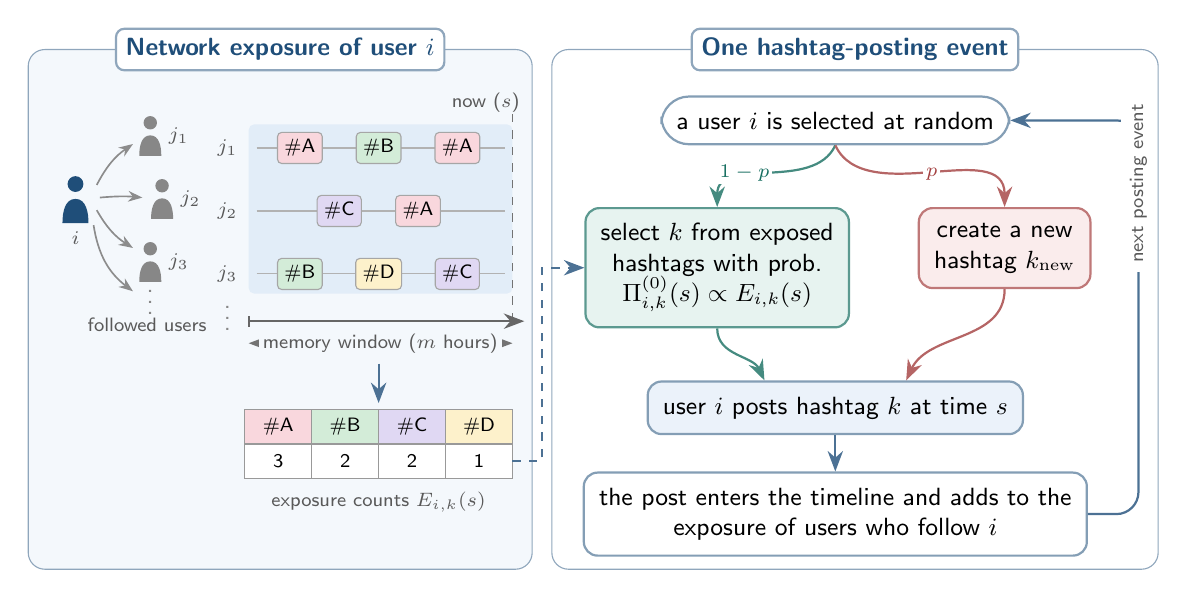
\begin{tikzpicture}[
  card/.style={draw=mainblue!55, thick, rounded corners=5pt, fill=postfill, align=center, font=\small, inner sep=5.5pt},
  startcap/.style={draw=mainblue!55, thick, rounded corners=10pt, fill=white, align=center, font=\small, inner sep=5.5pt},
  tag/.style={draw=black!35, rounded corners=1.5pt, inner sep=2.5pt, font=\scriptsize},
  arr/.style={-{Stealth[length=2.6mm]}, thick, mainblue!80},
  darr/.style={-{Stealth[length=2.6mm]}, thick, mainblue!80, dashed},
  ttab/.style={fill=white, draw=mainblue!50, thick, rounded corners=3pt, font=\small\bfseries, text=mainblue, inner sep=3.5pt},
  note/.style={font=\scriptsize, text=black!65, align=center},
  person/.pic={
    \fill[#1] (0,0.12) circle (0.085);
    \fill[#1] (-0.14,-0.30) to[out=90,in=180] (0,-0.04) to[out=0,in=90] (0.14,-0.30) -- cycle;
  }
]
% ================= LEFT PANEL (same height as right) =================
\draw[draw=mainblue!50, fill=panelfill, rounded corners=6pt] (0.15,0.85) rectangle (6.55,7.45);
\node[ttab] at (3.35,7.45) {Network exposure of user $i$};

% --- network sketch ---
\pic[scale=1.18] at (0.75,5.6) {person=mainblue};
\node[note] at (0.75,5.05) {$i$};
\pic at (1.7,6.4) {person=grayuser};
\node[note] at (2.06,6.35) {$j_1$};
\pic at (1.85,5.6) {person=grayuser};
\node[note] at (2.21,5.55) {$j_2$};
\pic at (1.7,4.8) {person=grayuser};
\node[note] at (2.06,4.75) {$j_3$};
\draw[-{Stealth[length=1.8mm]}, semithick, black!45] (1.02,5.73) to[bend left=14] (1.48,6.25);
\draw[-{Stealth[length=1.8mm]}, semithick, black!45] (1.06,5.57) to[bend left=5] (1.6,5.57);
\draw[-{Stealth[length=1.8mm]}, semithick, black!45] (1.02,5.41) to[bend right=14] (1.48,4.93);
\node[font=\small, text=grayuser] at (1.7,4.34) {$\vdots$};
\draw[-{Stealth[length=1.8mm]}, semithick, black!45] (0.98,5.22) to[bend right=22] (1.48,4.38);
\node[note] at (1.66,3.95) {followed users};

% --- posts of followed users (band x 2.95--6.3) ---
\fill[windowfill, rounded corners=2pt] (2.95,4.35) rectangle (6.3,6.5);
\draw[dashed, black!55] (6.3,4.0) -- (6.3,6.65);
\node[note] at (5.96,6.77) {now ($s$)};

\node[note] at (2.68,6.2) {$j_1$};
\draw[black!30] (3.05,6.2) -- (6.2,6.2);
\node[tag, fill=tagA] at (3.6,6.2) {\#A};
\node[tag, fill=tagB] at (4.6,6.2) {\#B};
\node[tag, fill=tagA] at (5.6,6.2) {\#A};
\node[note] at (2.68,5.4) {$j_2$};
\draw[black!30] (3.05,5.4) -- (6.2,5.4);
\node[tag, fill=tagC] at (4.1,5.4) {\#C};
\node[tag, fill=tagA] at (5.1,5.4) {\#A};
\node[note] at (2.68,4.6) {$j_3$};
\draw[black!30] (3.05,4.6) -- (6.2,4.6);
\node[tag, fill=tagB] at (3.6,4.6) {\#B};
\node[tag, fill=tagD] at (4.6,4.6) {\#D};
\node[tag, fill=tagC] at (5.6,4.6) {\#C};
\node[font=\small, text=grayuser] at (2.68,4.14) {$\vdots$};

% --- time axis ---
\draw[arr, black!60] (2.95,4.0) -- (6.45,4.0);
\draw[black!60, thick] (2.95,3.93) -- (2.95,4.07);
\draw[{Stealth[length=1.8mm]}-{Stealth[length=1.8mm]}, semithick, black!55] (2.95,3.72) -- (6.3,3.72);
\node[note, fill=panelfill, inner sep=1.5pt] at (4.62,3.72) {memory window ($m$ hours)};

% --- arrow to table ---
\draw[arr] (4.6,3.46) -- (4.6,2.96);

% --- exposure table (aligned with band) ---
\foreach \x/\t/\c/\v in {3.325/\#A/tagA/3, 4.175/\#B/tagB/2, 5.025/\#C/tagC/2, 5.875/\#D/tagD/1}{
  \draw[fill=\c, draw=black!40] (\x-0.425,2.44) rectangle (\x+0.425,2.88);
  \node[font=\scriptsize] at (\x,2.66) {\t};
  \draw[fill=white, draw=black!40] (\x-0.425,2.00) rectangle (\x+0.425,2.44);
  \node[font=\scriptsize] at (\x,2.22) {\v};
}
\node[note] at (4.6,1.70) {exposure counts $E_{i,k}(s)$};

% ================= RIGHT PANEL =================
\draw[draw=mainblue!50, rounded corners=6pt] (6.8,0.85) rectangle (14.5,7.45);
\node[ttab] at (10.65,7.45) {One hashtag-posting event};

\node[startcap] (start) at (10.4,6.55) {a user $i$ is selected at random};

\node[card, draw=adoptc!70, fill=adoptfill, anchor=north] (adopt) at (8.9,5.45) {select $k$ from exposed\\ hashtags with prob.\\ $\Pi^{(0)}_{i,k}(s)\propto E_{i,k}(s)$};
\node[card, draw=createc!70, fill=createfill, anchor=north] (create) at (12.55,5.45) {create a new\\ hashtag $k_{\mathrm{new}}$};

\draw[arr, adoptc!80] (start.south) to[out=-115,in=90] node[pos=0.45, left=1pt, font=\scriptsize, text=adoptc, fill=white, inner sep=1pt] {$1-p$} (adopt.north);
\draw[arr, createc!80] (start.south) to[out=-65,in=90] node[pos=0.45, right=1pt, font=\scriptsize, text=createc, fill=white, inner sep=1pt] {$p$} (create.north);

\node[card] (post) at (10.4,2.9) {user $i$ posts hashtag $k$ at time $s$};
\draw[arr, adoptc!80] (adopt.south) to[out=-90,in=115] ([xshift=-9mm]post.north);
\draw[arr, createc!80] (create.south) to[out=-90,in=65] ([xshift=9mm]post.north);

\node[card, fill=white] (upd) at (10.4,1.55) {the post enters the timeline and adds to the\\ exposure of users who follow $i$};
\draw[arr] (post) -- (upd);

\draw[darr] (6.3,2.22) -- (6.67,2.22) |- (adopt.west);

\draw[arr, rounded corners=8pt] (upd.east) -- (14.25,1.55) -- (14.25,6.55) -- (start.east);
\node[fill=white, rotate=90, font=\scriptsize, text=black!65] at (14.25,5.75) {next posting event};
\end{tikzpicture}
\end{document}
